\documentclass[tikz]{standalone}


% Codice per lo stile della freccia
\pgfarrowsdeclare{freccia45}{freccia45}
{
  \pgfarrowsleftextend{0pt}
  \pgfarrowsrightextend{\pgfgetarrowoptions{freccia45}+1.307\pgflinewidth}
}
{
  \pgfmathsetlengthmacro{\lun}{\pgfgetarrowoptions{freccia45}/cos(22.5)}
  \pgfsetdash{}{+0pt}
  \pgfsetmiterjoin
  \pgfpathmoveto{\pgfpointadd{\pgfqpoint{\pgfgetarrowoptions{freccia45}}{0pt}}{\pgfqpointpolar{157.5}{\lun}}}
  \pgfpathlineto{\pgfqpoint{\pgfgetarrowoptions{freccia45}}{0pt}}
  \pgfpathlineto{\pgfpointadd{\pgfqpoint{\pgfgetarrowoptions{freccia45}}{0pt}}{\pgfqpointpolar{-157.5}{\lun}}}
  \pgfpathclose
  \pgfusepathqstroke
}
\def\miodef{0.4cm} % imposta il valore utilizzato per default
\pgfsetarrowoptions{freccia45}{\miodef} % valore utilizzato se /punta non viene invocato
\pgfkeys{/punta/.default=\miodef, /punta/.code={\pgfsetarrowoptions{freccia45}{#1}}}

\usetikzlibrary{arrows,shapes}
\begin{document}
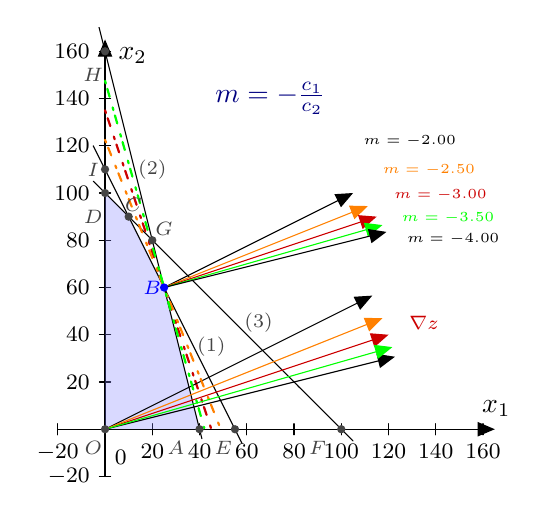
\begin{tikzpicture}[line cap=round,line join=round,>=triangle 45,x=0.03cm,y=0.03cm]
\definecolor{ffqqtt}{rgb}{1,0,0.2}
\definecolor{ccqqqq}{rgb}{0.8,0,0}
\definecolor{ttqqqq}{rgb}{0.2,0,0}
\definecolor{uuuuuu}{rgb}{0.27,0.27,0.27}
\definecolor{qqqqff}{rgb}{0,0,1}
\draw[->,color=black] (-20,0) -- (165,0);
\foreach \x in {-20,20,40,60,80,100,120,140,160}
\draw[shift={(\x,0)},color=black] (0pt,2pt) -- (0pt,-2pt) node[below] {\footnotesize $\x$};
\draw[color=black] (155.54,1.27) node [anchor=south west] {$x_1$};
\draw[->,color=black] (0,-20) -- (0,165);
\foreach \y in {-20,20,40,60,80,100,120,140,160}
\draw[shift={(0,\y)},color=black] (2pt,0pt) -- (-2pt,0pt) node[left] {\footnotesize $\y$};
\draw[color=black] (1.63,158.35) node [anchor=west] {$x_2$};
\draw[color=black] (0pt,-10pt) node[right] {\footnotesize $0$};
\clip(-20,-20) rectangle (180,170);

\fill[color=blue!50!white,opacity=0.3] (0,0)--(40,0)--(25,60)--(10,90)--(0,100)--cycle; %,pattern=north west lines
% vincolo 1
  \draw [domain=-5:58] plot(\x,{(--2200-40*\x)/20});
% vincolo 2
  \draw [domain=-5:41] plot(\x,{(--320-8*\x)/2});
% vincolo 3
  \draw [domain=-5:105] plot(\x,{(--100-1*\x)/1});
% gradiente
  \draw [->,color=ccqqqq] (0,0) -- (120,40);
% isoprofitto <= 5400
  \draw [line width=0.8pt,dash pattern=on 1pt off 2pt on 3pt off 4pt,color=ccqqqq,domain=0:45] plot(\x,{(-5400--120*\x)/-40});

  \draw [->,color=black] (0,0) -- (113.12, 56.56);
  \draw [->,color=black] (0,0) -- (122.72, 30.68);

% 2.25	116.25
% 2.5	122.5
% 2.75	128.75  
%  \draw [->,color=yellow] (0,0) --(115.60, 51.36); % 2.25
%  \draw [line width=0.8pt,dash pattern=on 1pt off 2pt on 3pt off 4pt,color=yellow,domain=0:52] plot(\x,{(-2.25*\x+116.25)});
  
  \draw [->,color=orange] (0,0) --(117.44, 47.00); % 2.5
  \draw [line width=0.8pt,dash pattern=on 1pt off 2pt on 3pt off 4pt,color=orange,domain=0:49] plot(\x,{(-2.5*\x+122.5)});
  
%  \draw [->,color=red] (0,0) --   (118.88, 43.24);
%  \draw [line width=0.8pt,dash pattern=on 1pt off 2pt on 3pt off 4pt,color=red,domain=0:47] plot(\x,{-2.75*\x+128.75});

  
% 3.25	141.25
% 3.5	147.5
% 3.75	153.75
%  \draw [->,color=lime] (0,0) --   (120.88, 37.2);
%  \draw [line width=0.8pt,dash pattern=on 1pt off 2pt on 3pt off 4pt,color=lime,domain=0:44] plot(\x,{-3.25*\x+141.25});
  \draw [->,color=green] (0,0) --(121.64, 34.76);
  \draw [line width=0.8pt,dash pattern=on 1pt off 2pt on 3pt off 4pt,color=green,domain=0:42] plot(\x,{-3.5*\x+147.5});
%  \draw [->,color=blue] (0,0) --(122.24, 32.6);
%  \draw [line width=0.8pt,dash pattern=on 1pt off 2pt on 3pt off 4pt,color=blue,domain=0:41] plot(\x,{-3.75*\x+153.75});
  
%%%%%%%%%%%%%%%%%%

\draw[color=blue!50!black] (70,140) node {$m=-\frac{c_1}{c_2}$};

\tiny{
\draw [->,color=black] (25,60) --(105.00, 100.00);
\draw[color=black] (129.00,122.00) node {$m = -2.00$};
%\draw [->,color=yellow] (25,60) --(108.51, 97.11);
%\draw[color=yellow] (133.56,115.75) node {$m = -2.25$};
\draw [->,color=orange] (25,60) --(111.21, 94.48);
\draw[color=orange] (137.07,109.83) node {$m = -2.50$};
%\draw [->,color=red] (25,60) --(113.32, 92.12);
%\draw[color=red] (139.82,104.25) node {$m = -2.75$};
\draw [->,color=ccqqqq] (25,60) --(115.00, 90.00);
\draw[color=ccqqqq] (142.00,99.00) node {$m = -3.00$};
%\draw [->,color=lime] (25,60) --(116.35, 88.11);
%\draw[color=lime] (143.76,94.04) node {$m = -3.25$};
\draw [->,color=green] (25,60) --(117.45, 86.42);
\draw[color=green] (145.19,89.34) node {$m = -3.50$};
%\draw [->,color=blue] (25,60) --(118.36, 84.90);
%\draw[color=blue] (146.37,84.87) node {$m = -3.75$};
\draw [->,color=black] (25,60) --(119.12, 83.53);
\draw[color=black] (147.35,80.59) node {$m = -4.00$};
}
%%%%%%%%%%%%%%%%%%
  
\begin{scriptsize}
% punto O
  \fill [color=uuuuuu] (0,0) circle (1.5pt);
  \draw[color=uuuuuu] (-5,-8) node {$O$};
% punto E
  \fill [color=uuuuuu] (55,0) circle (1.5pt);
  \draw[color=uuuuuu] (50,-8) node {$E$};
% punto I
  \fill [color=uuuuuu] (0,110) circle (1.5pt);
  \draw[color=uuuuuu] (-5,110) node {$I$};
% punto A
  \fill [color=uuuuuu] (40,0) circle (1.5pt);
  \draw[color=uuuuuu] (30,-8) node {$A$};
% punto H
  \fill [color=uuuuuu] (0,160) circle (1.5pt);
  \draw[color=uuuuuu] (-5,150) node {$H$};
% punto B
  \fill [color=qqqqff] (25,60) circle (1.5pt);
  \draw[color=qqqqff] (20,60) node {$B$};
  \fill [color=uuuuuu] (100,0) circle (1.5pt);
  \draw[color=uuuuuu] (90,-8) node {$F$};
  \fill [color=uuuuuu] (0,100) circle (1.5pt);
  \draw[color=uuuuuu] (-5,90) node {$D$};
  \fill [color=uuuuuu] (10,90) circle (1.5pt);
  \draw[color=uuuuuu] (12,95) node {$C$};
  \fill [color=uuuuuu] (20,80) circle (1.5pt);
  \draw[color=uuuuuu] (25,85) node {$G$};
  \draw[color=ccqqqq] (135,45) node {$\nabla z$};
  
  \draw[color=uuuuuu] (45, 35) node {$(1)$};
  \draw[color=uuuuuu] (20,110) node {$(2)$};
  \draw[color=uuuuuu] (65, 45) node {$(3)$};
\end{scriptsize}
\end{tikzpicture}
\end{document}